%!TEX root = ../thesis_a4.tex
\chapter{A Musicological Overview of Electronic Dance Music}
\label{chap:dancemusic}

\acrfull{edm} is a highly repetitive and rhythm-centric genre based on the liberal use of looping motifs consisting of layers of sampled and synthesised sound sources. Obviously, it is a style that is primarily intended for dance, at clubs, organised but illegal gatherings known as "raves" and large festivals but, as we will see, as the movement has evolved, that distinction has become quite blurred. In terms of nomenclature, it is often referred to as dance music or simply "dance" by its proponents (and opponents) in anglophonic Europe. Its abbreviation, \acrshort{edm}, as Reynolds - a music culture author and researcher who has been reporting on dance culture for many years - notes, seems to be a North American labelling that has been applied to a marked resurgence in dance music over the past decade primarily in the United States\footnote{\url{https://www.theguardian.com/music/2012/aug/02/how-rave-music-conquered-america}}. For the purposes of this thesis I will use the term dance music, as it is what I have always called it. Should there be ambiguity between electronic dance music and say, dance forms from Western Art music or folk, I will make the necessary distinctions clear.

Dance music is made up of a bewildering taxonomy of deeply branched sub-genres that are defended rigorously by their disciples with an almost religious fervour. A glance at Ishkur's excellent online resource "Ishkur's Guide to Electronic Music" \footnote{\url{http://techno.org/electronic-music-guide/}}
(\figref{fig:ishkur}) reveals 7 high level strands that include "House", "Trance", "Techno", "Breakbeat", "Jungle", "Hardcore" and "Downtempo"\footnote{A more formal catalogue is presented by McLeod (2001), but Ishkur’s guide is infamous enough to be referenced by many other articles in serious literature
\citep{leimeister2014rhythmic, Pampalk2005}.}. Within House, for example, we can see a complicated network of arches tracing its genesis from other non-electronic dance music specific genres in the 1970s (e.g. disco) to its many different modern incarnations. 

Three of these top level sub-genres are what we would deem representative and ambassadorial in describing dance music, namely techno, house and jungle, and we will expand on each of them now in turn, followed by some remarks on another interesting direction in electronic music that defies easy categorisation.

\begin{figure}
	\begin{center}
		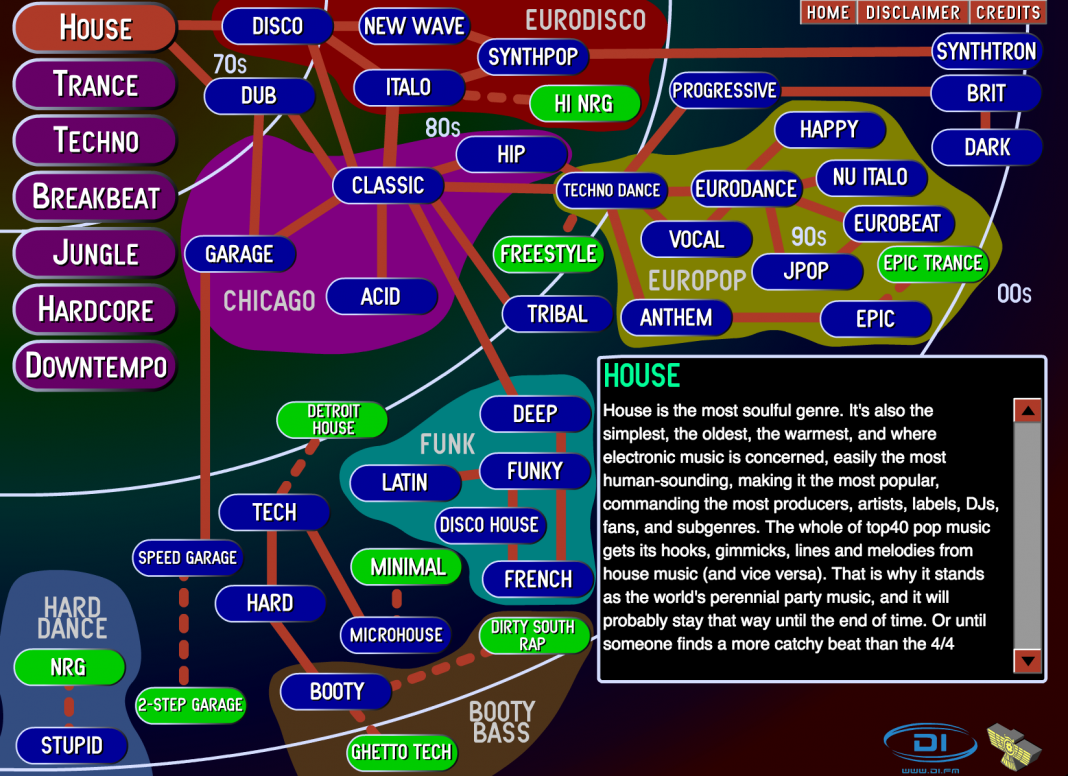
\includegraphics[width=\figSizeHundred]{ch02_dancemusic/figures/ishkur.png}
	\end{center}
	\caption[Ishkur's Guide to Electronic Music]{Ishkur's Guide to Electronic Music}
	\label{fig:ishkur}
\end{figure}

\section{House}

The act of going to a venue purely to dance and listen to recorded music carefully selected by a DJ existed well before the arrival what we now know as electronic dance music, as is clear from the disco era in the 1970s. Clubs such as “Paradise Garage” and “Studio 54” became focal points for the general public as well as artists living in New York, and were revered for their sound systems and resident music selectors. It was at these lengthy sessions that the cult of the DJ would nurture, with one of the most notable emerging being DJ Larry Levan. Levan would pioneer many aspects of what is now understood as the classic “DJ Set”, and was particularly celebrated for his ability to “read the crowd” - to adapt and change his sequencing and mixing depending on the mood of the audience of a given night. He was instrumental in developing the practice of remixing music, and in later years started to incorporate samplers and drum machines when repurposing older R\&B records for his dance floor.

The enduring legacy of disco left the most lasting impression on the city of Chicago, where it enjoyed heavy rotation in its venues long after its demise in other urban centres \citep{Reynolds2013}. Disco’s fading popularity meant that new releases were less forthcoming, inevitably leading DJs in the city scrambling to remix and update existing records à la Larry Levan, in order to stay fresh and current for audiences. One of Levan’s disciples, Frankie Knuckles, was a resident at the Warehouse club in Chicago, where his blending of regular disco and the electronic leaning Italo-disco from Italy (Giorgio Moroder would be its most notable export) soon became morphed and intertwined with his own bass lines and drum tracks \citep{Butler2006}. Eponymously, the name for this style was eventually shortened to become what is now known as ``house''.

Listening to classic house tracks, it is rooted unequivocally in a ``four on the floor'' regular 4/4 bass drum pattern, supplanted with synthesised claps and snares on the second and fourth backbeats, indicative of the equipment it was built on: the infamous TR-808 drum machine (\figref{fig:roland})\citep{Blashill2002}. Owing to its disco roots, house music is often described as the most “soulful” of dance music styles, in no small part due to syncopated baselines based around the root and the fifths, with short, jazzy electric piano style vamps providing harmonic context for catchy vocal hooks.

\begin{figure}
	\begin{center}
		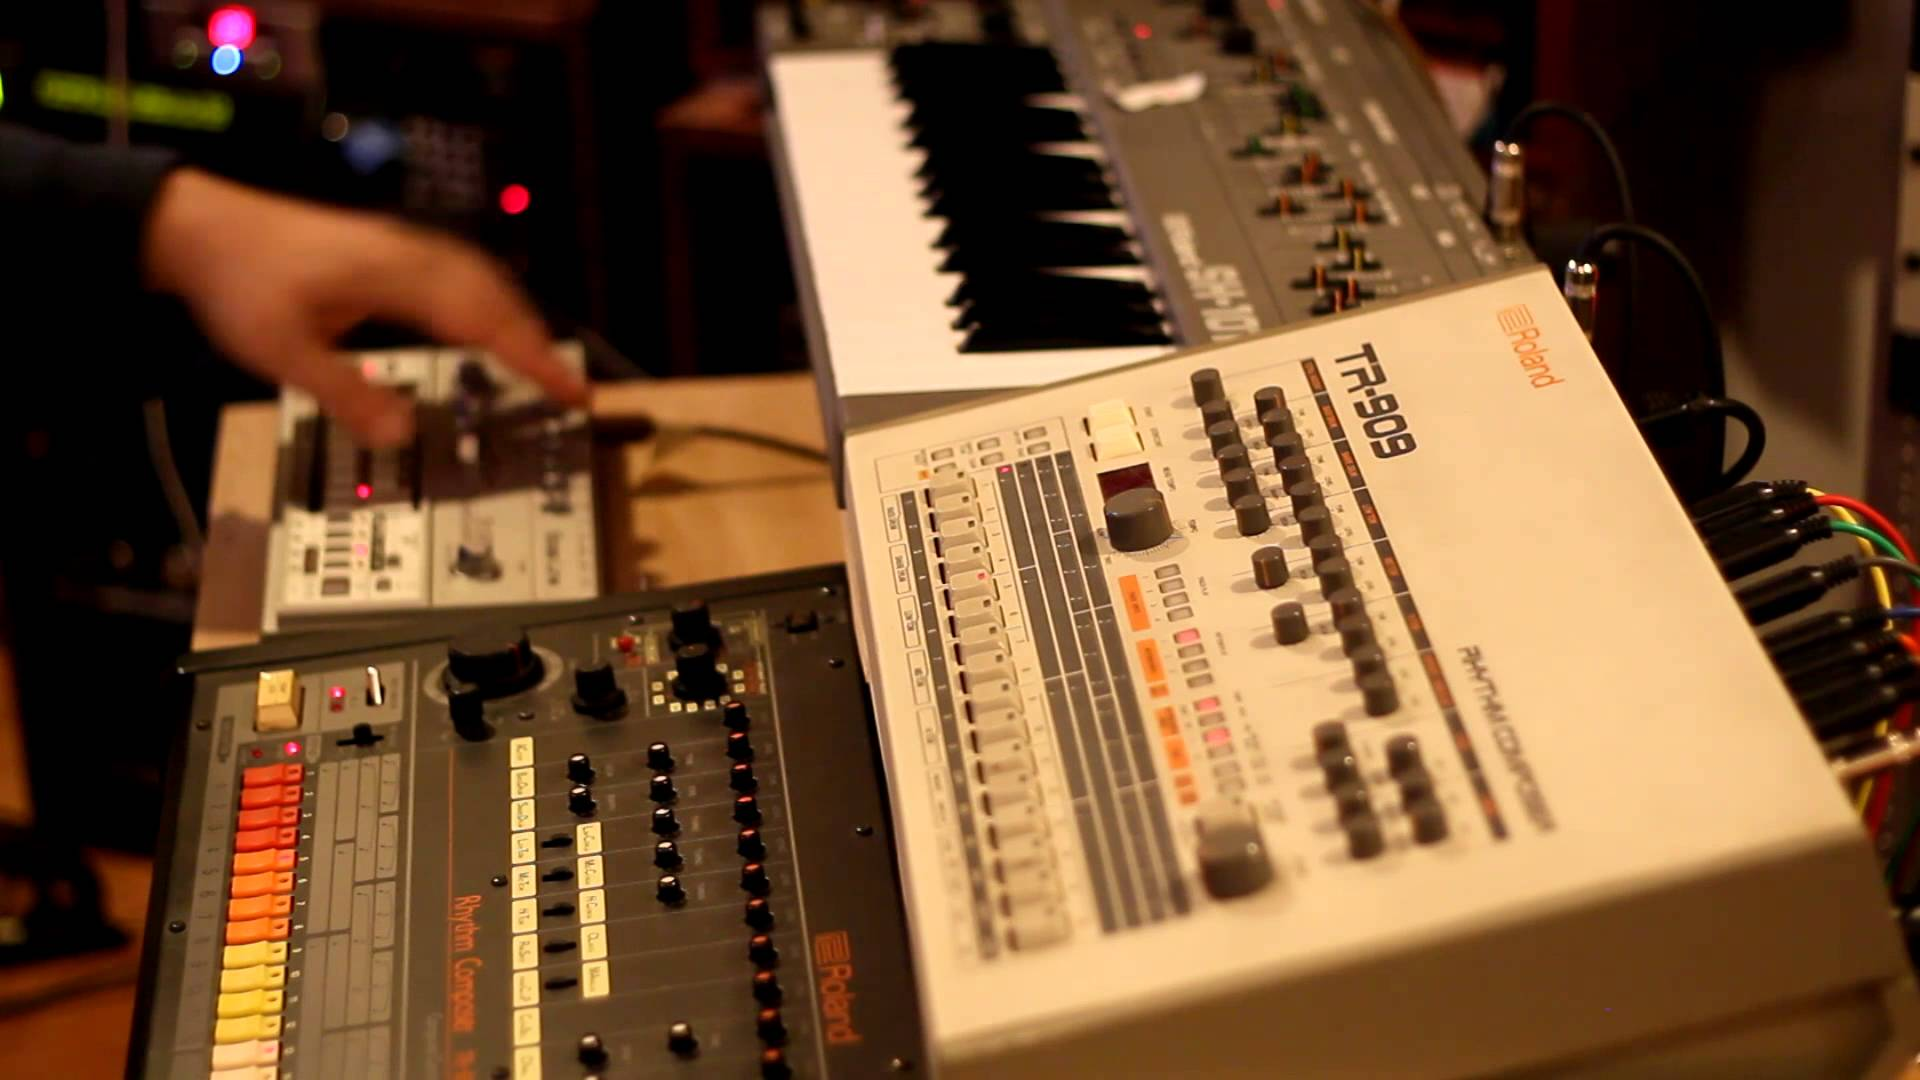
\includegraphics[width=\figSizeHundred]{ch02_dancemusic/figures/roland.jpg}
	\end{center}
	\caption[Roland Electronic Music Instruments]{The Roland Tr-303 (top-left), TR-808 (bottom-left) and TR-909 (bottom-right) (Image from Synth Mania)}
	\label{fig:roland}
\end{figure}

Towards the latter half of the 80s, the Chicago house scene gave way to a more stripped back, harder sound known as acid house. A classic example of how a singular misuse of technology can redefine an entire genre, acid house built its entire identity out of another Roland product, this time the TR-303 bass synthesiser \citep{McLeod2001}\footnote{\url{https://youtu.be/TLQwwtjtiY4}}. The production team “Phuture” discovered that by constantly modulating the frequency cutoff and resonance parameters of the bass pattern, they managed to create a frantic new “squelching” bass sound that both diminished the roles of traditional layering techniques using keys and vocals and emphasised the value of new production tricks, deliberate or accidental \citep{Vitos2014}. 

Acid house was to prove most influential, however, when the first records made their way across the Atlantic to the United Kingdom. In London and Manchester clubs such as Shroom and the Hacienda (the latter owned and managed by the label Factory Records along with its flagship group New Order \citep{hook2009hacienda}) heavy rotation of acid house tracks triggered what would eventually become known as the “rave” movement. The rave movement was centred around large, spontaneous but entirely unlicensed gatherings focussed on marathon sessions of dancing to acid house and, much to the chagrin of authorities, consumption of club drugs such as MDMA. Rave culture would reach its peak during 1988-1989, culminating in what is now referred to as the “Second Summer of Love” \citep{Gore1997}. High profile coverage in the tabloid newspapers caused `moral panic' \citep{Martin1999}, and demonised and politicised rave music, so much so that the controversial 1994 Criminal Justice Act included a clause granting police full authority to halt any event involving the “emission of a succession of repetitive beats” \citep{gilbert1997soundtrack} \footnote{Veteran duo Autechre (who could hardly ever be accused of basking in repetitivity) in response released \textit{Anti} EP containing a track ``programmed in such a way that no bars contain identical beats'', with the warning: ``...we advise DJs to have a lawyer and a musicologist present at all times to confirm the non-repetitive nature of the music in the event of police harassment'' \citep{Atkinson2007}} .

\section{Techno}

Around the end of the 1980s a similar musical development to house was burgeoning in the city of Detroit, Michigan. Detroit was already a complicated city with a chequered past; it was here that Motown records was formed, with artists like Marvin Gaye producing some of the most defining soul music of the 1960s and early 1970s. The name Motown, a portmanteau of motor and town,  acknowledges Detroit  as the “motor city” - once the epicentre for the American car industry in the early part of the 20th century. Towards the second half of the century this once booming complex collapsed due to increased overseas competition from countries like Japan and national economic decline. Today the graveyard of abandoned factories in downtown Detroit serve as a bitter reminder of these greater years \citep{Sicko2010}.

The continued de-industrialisation, suburbanisation and the eventual relocation of the legendary soul label Motown Records to Los Angeles in 1972 had a devastating impact on the cultural output of the urban centre. But bubbling under the surface in Detroit's suburbs three middle class African American high school friends, known as the “Belleville Three”,  were planting the seeds for what would become techno. Juan Atkins, Derrick May and Kevin Saunderson were obsessed with sci-fi, technology and futurism, and raised on a diet of George Clinton funk and Italo-disco coupled with frequent visits to Chicago for injections of house, however it is widely acknowledged that their greatest influence would be German electronic group Kraftwerk \citep{Pope2011}. This was largely due to a seminal local radio show hosted by Charles Johnson a.k.a. “The Electrifying Mojo”\footnote{\url{http://daily.redbullmusicacademy.com/2015/05/electrifying-mojo-feature}}, mixing artists like Prince with European new wave, italo-disco and krautrock \citep{Reynolds2013, Sicko2010}. But it’s no coincidence Atkins, May and Saunderson latched on to Kraftwerk forthright. Kraftwerk’s albums revealed a group enamoured with the themes of transport, progress and movement, from the Beach Boys inspired ode to German motorways  “Autobahn”, to the pan-European romanticism of rail travel on \textit{Trans-Europe Express} \citep{Albiez2010}. This naturally resonated with the Detroit trio’s formulating ideas of Afro-futurism, against the backdrop of a city once so intertwined with the machinery of transportation and automobilisation.

Like Chicago house, Detroit techno was constructed and produced using the tools available at the time, inevitably the gamut of Roland’s drum machines and bass sequencers, coupled with whatever other synthesisers and sampling equipment was on hand. Tempo markings are also similar than house, most frequently in the 110 to 140 bpm range. So what distinguishes techno from house then? Techno at least, is considered more minimal and mechanical than house, less rooted in the more soulful influences of disco and soul as artist May points out:  

\blockcquote[]{collins_schedel_wilson_2013}{``\textit{House still has its heart in 70s disco; we don’t have any of that respect for the past, it’s strictly future music. We have a much greater aptitude for experiment.}''}

There is a driving energy to techno that discriminates it from house tracks, the tonality is often more dissonant and ominous. Kraftwerk style vocoder driven vocals and titles such as “No UFO’s” [sic] and “Time Space Transmat” highlight the futurist, utopian themes and aesthetic that makes this era of Detroit techno idiosyncratic. 

Techno would go full circle and transport itself back to Germany, where clubs such as Tresor and Berghain in the capital of Berlin soon became shrines for techno lovers from around the world. Berlin takes its techno very seriously. Tresor and Berghain are housed in huge, imposing former power plants\footnote{Suffice it to say, Kraftwerk is the German word for “power station”} and factory warehouses, with the latter recently receiving the same tax status\footnote{\url{http://pitchfork.com/news/68211-berghain-declared-high-culture-venue-by-berlin-court/}} as other more historic cultural centres such as opera and concert halls \footnote{Berghain’s legal representative successfully argued that “concertgoers may achieve a similar intoxicating effect from a Mahler symphony as from a DJ set”}. These industrial settings have moulded and shaped the sound of techno further, just like acid house did with its softer earlier incarnations. German techno sounds big, heavy and dark. Kick drums are brutal, relentless and reverberated, the reliance is more on metallic, machinery inspired sound design than on any easily discernable pitched, melodic or harmonic material. \cite{Nye2013} has also traced this trajectory of evolution (or perhaps devolution?) and observes a marked `minimalism' of the sound compared to its trans-Atlantic predecessor.

\begin{figure}
	\begin{center}
		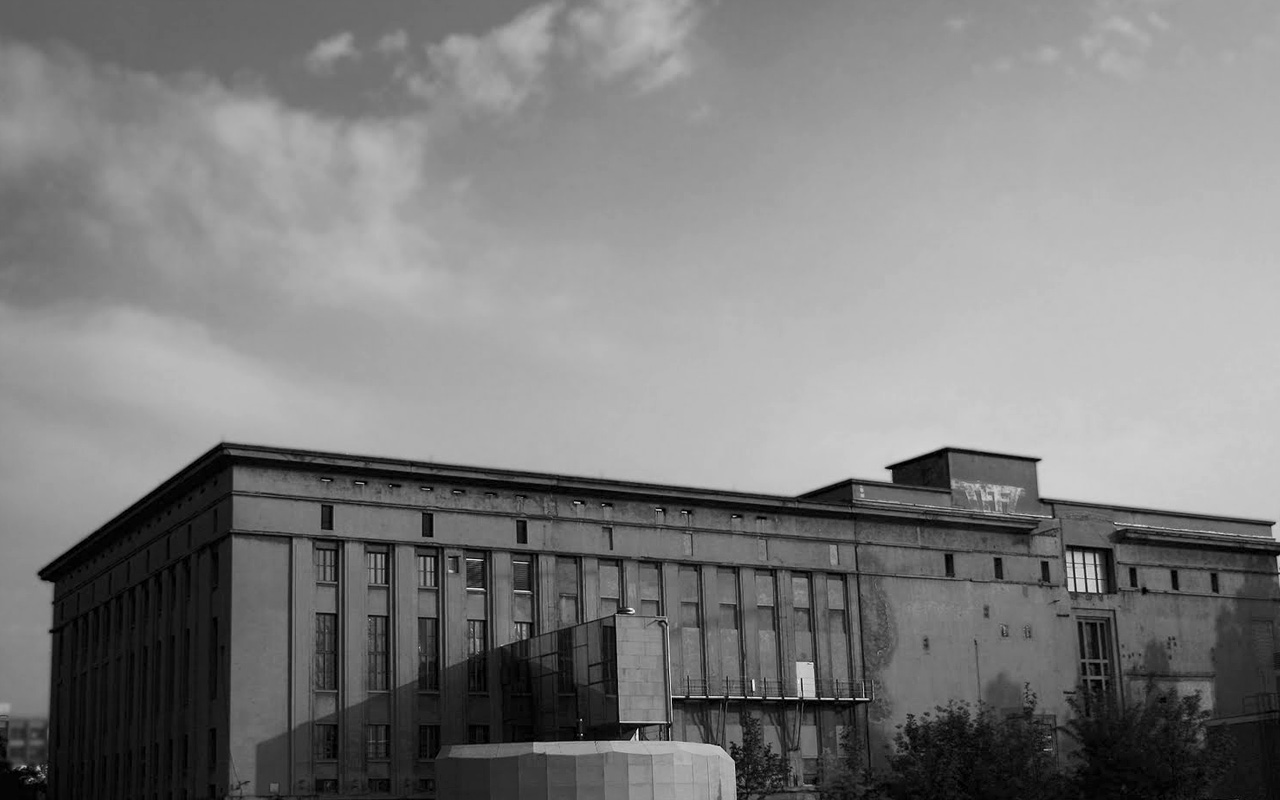
\includegraphics[width=\figSizeHundred]{ch02_dancemusic/figures/berghain.jpg}
	\end{center}
	\caption[Berghain Club in Berlin]{Berghain Club in Berlin, housed in a former power plant (Image from Resident Advisor)}
	\label{fig:roland}
\end{figure}

In a fitting closing observation, it is interesting to note that Kraftwerk, many years later, have acknowledged their influence on techno as well as the cultural duality shared by these two cities seemingly so far apart: on their track “Planet der Visionen” the refrain is \textit{"Detroit/Germany/We're so electric"}.

\section{Jungle and Drum ‘n’ Bass}

As the innocence and hope of rave dream started to disentangle and disintegrate in an increasingly volatile post-Thatcherite Britain, a radically new sound rose up from the ashes. Jungle, hardcore or drum ‘n’ bass drew its inspiration from two rather disparate influences. Firstly, in New York in the 1970s, DJ Kool Herc realised that by sequencing two copies of the same record, and looping the isolated “break” section - a short passage of drum soloing from funk and R\&B records - he could create a 5 minute performance for the purposes of “break” dancing and for an MC (Master of Ceremonies or Microphone Controller) to rhyme over \citep{Smith2000}. 

As such, Kool Herc essentially devised the underpinnings of a musical framework for emerging hip hop culture and rap music. Hip hop, as opposed to say, house and techno, is \textit{sample-oriented} music, meaning that manipulation of existing recordings of audio are utilised far more than raw signal generating synthesisers. Jungle builds on hip hop’s sampling aesthetic and heavy reliance on breaks but takes it to completely new extremes. With the development of sophisticated hardware production tools such as the Roland MPC (Music Production Centre) and, subsequently, the personal computer, endless new possibilities for complex and finely grained sample manipulation was within reach of homegrown bedroom producers.

Jungle’s other roots is the direct result of United Kingdom’s past as a colonial power. Migration from the Commonwealth Caribbean island of Jamaica\footnote{In fact, DJ Kool Herc was born in Kingston, Jamaica, and would have been exposed to dancehall culture before emigrating to the United States at the age of 12 \citep{Chang2007}.} to London brought with it reggae, dub music and sound system culture in general. Dub reggae was already a technology-centred form of music way before dance producers began twiddling with Roland gear. Engineers like Lee Scratch Perry would take instrumental versions of reggae tracks and remix them live using a slew of mixing desk tricks and exaggerated drenching of outboard effects (most prominently using the Roland Space Echo), blurring the lines between what constitutes the boundaries of the producer, performer and composer. Dub was performed at dedicated events with massive sound systems and MCs, somewhat prototypically anticipating central aspects of hip hop and rave. 

Just as reggae’s basic rhythm inverted the traditional downbeat and upbeat pattern of rock, jungle completely upends the traditional symmetry and repetition of house/techno dance music. Equally, just as the combined rhythm section of the bass guitar and drums (referred to as the \textit{riddim}) takes a more pivotal role in reggae, the drums in jungle and drum and bass are easily the most dominant element. As Simon Reynolds observes:

\blockcquote[]{Reynolds2013}{``\textit{In jungle, the rhythm is the melody; the drum patterns are as hooky as the vocal samples or keyboard refrains}''}

Where jungle departs greatly from its spiritual predecessor however is the actual arrangement of rhythmic patterns and its tempo. Reggae songs like chugs along typically around the 80 BPM mark; jungle can easily reach BPMs of almost double that\footnote{And wreaking havoc on BPM detectors!}. Drum production in jungle music is based around creating endlessly complex and dizzyingly intricate resequencing and reinterpretations of breakbeats. Many breakbeat samples have been used over the past decades, but the most infamous and enduring undoubtedly remains the “Amen Break”, a short 4-6 second drum solo on the song ``Amen Brother" by 1960s R\&B group The Winstons \citep{Collins2007a}. Along with an excerpt from ``Funky Drummer" by James Brown, they hold the contentious titles of being the most sampled breaks in music, contentious because the artists in question have received little or no royalty payments for its reproduction.

\section{Warp Records and \textit{Artificial Intelligence}}

By the early 1990s electronic dance music was already maturing to a point where it began to look inward at itself in reflection and contemplation. After a long night of hedonism, ravers were not likely to listen to more punishing dancefloor oriented beats but rather sought out a more subdued, laid back sound to match abating moods.

Warp Records, a Sheffield-based techno label anticipated this development and decided to capitalise on the emerging trend in a defining series of compilations known as \textit{Artificial Intelligence}. Looking at the green cover of the first release, it depicts a lone automaton comfortably seated in an armchair, facing a stereo system and a shelf of vinyl records. The intention is clear: this is not music for dancing, and as if the image wasn’t enough, the subtitle below proclaims “Electronic Listening Music From Warp”. The \textit{Artificial Intelligence} series would go on to release seven other albums, proving highly influential in the trajectory of dance music and bolstering Warp Records’ reputation as a bastion for “groundbreaking music” and, later on, branching into video and cinema. They cleverly managed to usher in an era of album format electronica, thus securing their longevity by doing away with the single release model responsible for the short lifespan of many a prior dance music imprint.

\begin{figure}
	\begin{center}
		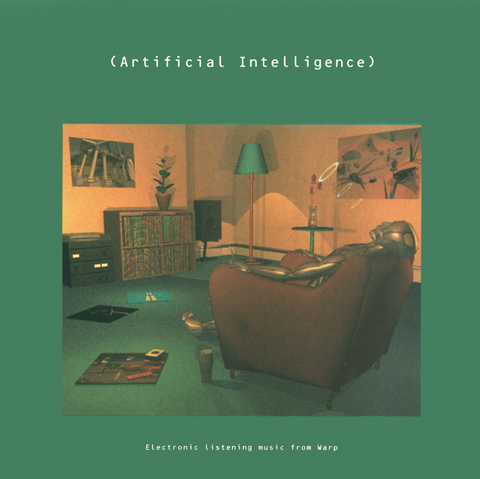
\includegraphics[width=0.6\textwidth]{ch02_dancemusic/figures/warp.jpg}
	\end{center}
	\caption[Cover Sleeve for Artificial Intelligence]{Cover Sleeve for Warp Records' \textit{Artificial Intelligence} (Image from Warp.net)}
	\label{fig:roland}
\end{figure}

The early music released by Warp Records was swiftly retitled by fans as \acrfull{idm}, a catch all label that largely grew out of discourse between members of Usenet forums discussing rave music to describe “music that moves the mind, not just the body” \citep{Alwakeel2009}. Immediately the term was controversial, even by those who would be considered its most respected innovators.  The problem with the IDM label is that it not so much describes a sound, rather than a collective ethos that just simply eschews conventional dancefloor geared sounds and production aesthetic. Richard D. James (Aphex Twin) takes further umbrage at the supposed elitist connotations it conveys:

\blockcquote[]{Haworth2015}{``\textit{I just think it's really funny to have terms like that. It's basically saying 'this is intelligent and everything else is stupid.' It's really nasty to everyone else's music. It makes me laugh.}''}

Comparing Warp Records’ stalwart roster of Aphex Twin, Squarepusher, Autechre and Boards of Canada under this umbrella term proves how divisive and varied the actual musical output is. Scottish duo Boards of Canada blend an uneasy mix of woozy, tape modulated hip hop beats with nostalgic samples from old VHS cassettes on their classic albums \textit{Music Has The Right To Children} and \textit{Geogaddy}. This is light years removed from, for example, the increasingly cold, angular and austere precision that has characterised most of Autechre’s exhaustive back catalogue. Starting out with reasonably symmetric post-techno repetitions and melodic analog synthesis on albums like \textit{Incunabula} and \textit{Tri Repetae}, Autechre’s music has become more abstract and hard to pin down over time, owing as much sonically and aesthetically to Greek composer/theorist Iannis Xenakis as to any Detroit pioneer.

Mostly this transformation has arisen out of their shifting and maturing use of technology. Albums like \textit{Confeld} betray a pair of experimentalists enamored with algorithmic composition, particularly using the Max/MSP environment. Regarding their continuing use of interactive software in live contexts they have described\footnote{\url{https://www.residentadvisor.net/features/2756}} how their processes differ from more traditional laptop performances: 

\blockquote{``\textit{I mean, there's no actual music "there"—it's not like we make music, then use the system to replay it in new ways. The system itself is making the music each time, it's all about the capabilities of the system dictating what the music's like}''}

Indisputably however, it is Aphex Twin who has become the bona fide poster boy for Warp Records and IDM as a whole. The Cornish producer started out with two double albums exploring ambient techno and beatless ambient music on \textit{Selected Ambient Works 85–92} and \textit{Selected Ambient Works Volume II} respectively. Later albums delved further into extreme recontextualisation and interpretation of earlier jungle and drum ‘n’ bass - often referred to by its detractors as “drill ‘n’ bass” due to its harshness and intensity - culminating in his most personal and broad record: \textit{Drukqs}. Over two discs, this album leaps from Satie-esque furniture music on “Avril 14th” to musique concrète (``Gwarek2'', ``Gwety Mernans''), as well his many brutally complex post jungle workouts on tracks like “Vordhosbn” and “Mt Saint Michel + Saint Michaels Mount”. 

Richard D. James and his labelmates, with their supposed ``intelligent" take on dance music, managed to win much favour and legitimacy in contemporary and art music circles. The 2006 compilation \textit{Warp Works \& Twentieth Century Masters }mixed pieces of Aphex Twin and Squarepusher pieces alongside performances of Ligeti, Varèse and Cage, while London-based chamber ensemble Alarm Will Sound have recorded careful and faithful arrangements of Aphex Twin and Autechre on albums such as  \textit{A/Rhythmia}. What’s striking about listening to these experiments is how natural and appropriate they sound compared to many forced and kitsch attempts at orchestrating rock music for instance.\footnote{Perhaps this is more of a personal aversion - I played in orchestras in my youth and I absolutely loathed those light medley arrangements of Beatles and Beach Boys that sanctified all the dangerous elements of rock `n' roll.}

As suggested in the introductory chapter, this has been an attempt to provide a short familiarisation with dance music from cultural, musicological and, in places, sociopolitical perspectives. It was not my intention to be exhaustive nor authoritative; I understand there are countless subgenres of dance music that I have omitted for the sake of brevity and enthusiasts and experts alike may take umbrage with those I've chosen to retain and my summaries of them. What I would hope is that the reader gains a flavour of my understanding of dance music and appreciate its scope for our forthcoming study.